\documentclass{../../slides-style}

\slidetitle{Многопоточное программирование в F\#}{19.04.2024}

\begin{document}

    \begin{frame}[plain]
        \titlepage
    \end{frame}

    \section{Async}

    \subsection{Пример}

    \begin{frame}[fragile]
        \frametitle{Async workflow}
        \begin{footnotesize}
            \begin{minted}{fsharp}
open System.Net
open System.IO
let sites = ["http://se.math.spbu.ru"; "http://spisok.math.spbu.ru"]
let fetchAsync url =
    async { 
        do printfn "Creating request for %s..." url
        let request = WebRequest.Create(url)
        use! response = request.AsyncGetResponse()
        do printfn "Getting response stream for %s..." url
        use stream = response.GetResponseStream()
        do printfn "Reading response for %s..." url
        use reader = new StreamReader(stream)
        let html = reader.ReadToEnd()
        do printfn "Read %d characters for %s..." html.Length url 
    }

sites |> List.map (fun site -> site |> fetchAsync |> Async.Start) |> ignore
            \end{minted}
        \end{footnotesize}
    \end{frame}

    \begin{frame}[fragile]
        \frametitle{Что получится}
        \begin{alertblock}{F\# Interactive}
            \begin{minted}{fsharp}
Creating request for http://se.math.spbu.ru...
Creating request for http://spisok.math.spbu.ru...
val sites : string list =
  ["http://se.math.spbu.ru"; "http://spisok.math.spbu.ru"]
val fetchAsync : url:string -> Async<unit>
val it : unit = ()

> Getting response stream for http://spisok.math.spbu.ru...
Reading response for http://spisok.math.spbu.ru...
Read 4475 characters for http://spisok.math.spbu.ru...
Getting response stream for http://se.math.spbu.ru...
Reading response for http://se.math.spbu.ru...
Read 217 characters for http://se.math.spbu.ru...
            \end{minted}
        \end{alertblock}
    \end{frame}

    \subsection{Thread Pool}

    \begin{frame}[fragile]
        \frametitle{Переключение между потоками}
        Распечатаем Id потоков, в которых вызываются методы printfn:
        \begin{minted}{fsharp}
open System.Threading

let tprintfn fmt =
    printf "[.NET Thread %d]"   
        Thread.CurrentThread.ManagedThreadId;
    printfn fmt
        \end{minted}
    \end{frame}

    \begin{frame}[fragile]
        \frametitle{Что получилось теперь}
        \begin{footnotesize}
            \begin{alertblock}{F\# Interactive}
                \begin{minted}{fsharp}
[.NET Thread 47][.NET Thread 49]Creating request 
        for http://se.math.spbu.ru...
Creating request for http://spisok.math.spbu.ru...
val sites : string list =
  ["http://se.math.spbu.ru"; "http://spisok.math.spbu.ru"]
val tprintfn : fmt:Printf.TextWriterFormat<'a> -> 'a
val fetchAsync : url:string -> Async<unit>
val it : unit = ()

> [.NET Thread 49]Getting response stream for 
        http://spisok.math.spbu.ru...
[.NET Thread 49]Reading response for http://spisok.math.spbu.ru...
[.NET Thread 50]Getting response stream for http://se.math.spbu.ru...
[.NET Thread 50]Reading response for http://se.math.spbu.ru...
[.NET Thread 50][.NET Thread 49]Read 217 characters 
        for http://se.math.spbu.ru...
Read 4475 characters for http://spisok.math.spbu.ru...
                \end{minted}
            \end{alertblock}
        \end{footnotesize}
    \end{frame}

    \subsection{Async Workflow}

    \begin{frame}[fragile]
        \frametitle{Подробнее про Async}
        \framesubtitle{Async --- это Workflow}
        \begin{minted}{fsharp}
type Async<'a> = Async of ('a -> unit) * (exn -> unit) 
        -> unit

type AsyncBuilder with
    member Return : 'a -> Async<'a>
    member Delay : (unit -> Async<'a>) -> Async<'a>
    member Using: 'a * ('a -> Async<'b>) -> 
            Async<'b> when 'a :> System.IDisposable
    member Let: 'a * ('a -> Async<'b>) -> Async<'b>
    member Bind: Async<'a> * ('a -> Async<'b>) 
            -> Async<'b>
        \end{minted}
    \end{frame}

    \begin{frame}
        \frametitle{Какие конструкции поддерживает Async}
        \begin{ssmall}
            \begin{tabu} {| X[0.3 l p] | X[1 l p] |}
                \tabucline-
                Конструкция               & Описание           \\
                \tabucline-
                \everyrow{\tabucline-}
                let! pat = expr           & Выполняет асинхронное вычисление expr и присваивает результат pat, когда оно заканчивается   \\
                let pat = expr            & Выполняет синхронное вычисление expr и присваивает результат pat немедленно \\
                use! pat = expr           & Выполняет асинхронное вычисление expr и присваивает результат pat, когда оно заканчивается. Вызовет Dispose для каждого имени из pat, когда Async закончится.    \\
                use pat = expr            & Выполняет синхронное вычисление expr и присваивает результат pat немедленно. Вызовет Dispose для каждого имени из pat, когда Async закончится. \\
                do! expr                  & Выполняет асинхронную операцию expr, эквивалентно let! () = expr \\
                do expr                   & Выполняет синхронную операцию expr, эквивалентно let () = expr \\
                return expr               & Оборачивает expr в Async<'T> и возвращает его как результат Workflow \\
                return! expr              & Возвращает expr типа Async<'T> как результат Workflow \\
            \end{tabu}
        \end{ssmall}
    \end{frame}

    \subsection{Control.Async}

    \begin{frame}
        \frametitle{Control.Async}
        \framesubtitle{Что можно делать со значением Async<'T>, сконструированным билдером}
        \begin{ssmall}
            \begin{tabu} {| X[0.7 l p] | X[1 l p] | X[1 l p] |}
                \tabucline-
                Метод              & Тип                                         & Описание           \\
                \tabucline-
                \everyrow{\tabucline-}
                RunSynchronously   & Async<'T> * ?int * ?CancellationToken -> 'T                       & Выполняет вычисление синхронно, возвращает результат \\
                Start              & Async<unit> * ?CancellationToken -> unit                          & Запускает вычисление асинхронно, тут же возвращает управление \\
                Parallel           & seq<Async<'T> > -> Async<'T []>                                   & По последовательности Async-ов делает новый Async, исполняющий все Async-и параллельно и возвращающий массив результатов \\
                Catch              & Async<'T> -> Async<Choice<'T,exn> >                               & По Async-у делает новый Async, исполняющий Async и возвращающий либо результат, либо исключение \\
                StartImmediate     & Async<unit> * ?CancellationToken -> unit                          & Выполняет вычисление асинхронно в вызвавшем потоке \\
                StartAsTask        & Async<'T> * ?TaskCreationOptions * ?CancellationToken -> Task<'T> & Запускает вычисление и оборачивает его в Task \\
                AwaitTask          & Task<'T> -> Async<'T>                                             & Оборачивает Task в Async \\
            \end{tabu}
        \end{ssmall}
    \end{frame}

    \begin{frame}[fragile]
        \frametitle{Пример}
        \begin{minted}{fsharp}
let writeFile fileName bufferData =
    async {
      use outputFile = System.IO.File.Create(fileName)
      do! outputFile.AsyncWrite(bufferData) 
    }

Seq.init 1000 (fun num -> createSomeData num)
|> Seq.mapi (fun num value -> 
      writeFile ("file" + num.ToString() + ".dat") value)
|> Async.Parallel
|> Async.RunSynchronously
|> ignore
        \end{minted}
    \end{frame}

    \subsection{Исключения в Async}

    \begin{frame}[fragile]
        \frametitle{Подробнее про Async.Catch}
        \begin{minted}{fsharp}
asyncTaskX
    |> Async.Catch
    |> Async.RunSynchronously
    |> fun x ->
        match x with
        | Choice1Of2 result -> 
           printfn "Async operation completed: %A" result
        | Choice2Of2 (ex : exn) -> 
           printfn "Exception thrown: %s" ex.Message
        \end{minted}
    \end{frame}
    
    \begin{frame}[fragile]
        \frametitle{Обработка исключений прямо внутри Async}
        \begin{minted}{fsharp}
async {
    try
        // ...
    with
    | :? IOException as ioe ->
        printfn "IOException: %s" ioe.Message
    | :? ArgumentException as ae ->
        printfn "ArgumentException: %s" ae.Message
}
        \end{minted}
    \end{frame}

    \subsection{Отмена операций}

    \begin{frame}[fragile]
        \frametitle{Отмена операции}
        \framesubtitle{Задача, которую можно отменить}
        \begin{minted}{fsharp}
open System
open System.Threading

let cancelableTask =
    async {
        printfn "Waiting 10 seconds..."
        for i = 1 to 10 do
            printfn "%d..." i
            do! Async.Sleep(1000)
        printfn "Finished!"
    }
        \end{minted}
    \end{frame}

    \begin{frame}[fragile]
        \frametitle{Отмена операции}
        \framesubtitle{Код, который её отменяет}
        \begin{minted}{fsharp}
let cancelHandler (ex : OperationCanceledException) =
    printfn "The task has been canceled."

Async.TryCancelled(cancelableTask, cancelHandler)
|> Async.Start

// ...

Async.CancelDefaultToken()
        \end{minted}
    \end{frame}

    \begin{frame}[fragile]
        \frametitle{CancellationToken}
        \begin{minted}{fsharp}
open System.Threading

let computation = Async.TryCancelled(cancelableTask, 
        cancelHandler)
let cancellationSource = new CancellationTokenSource()

Async.Start(computation, cancellationSource.Token)

// ...

cancellationSource.Cancel()
        \end{minted}
    \end{frame}

    \subsection{Async.StartWithContinuations}

    \begin{frame}[fragile]
        \frametitle{Async.StartWithContinuations}
        \begin{minted}{fsharp}
Async.StartWithContinuations(
    someAsyncTask,
    (fun result -> printfn "Task completed with result %A" result),
    (fun exn -> 
        printfn "Task threw an exception with Message: 
                %s" exn.Message),
    (fun oce -> printfn "Task was cancelled. 
                Message: %s" oce.Message)
)
        \end{minted}
    \end{frame}

    \subsection{Async.AwaitEvent}

    \begin{frame}[fragile]
        \frametitle{Async.AwaitEvent}
        \begin{minted}{fsharp}
open System

let timer = new Timers.Timer(2000.0)
let timerEvent = Async.AwaitEvent (timer.Elapsed) 
    |> Async.Ignore

printfn "Waiting for timer at %O" DateTime.Now.TimeOfDay
timer.Start()

printfn "Doing something useful while waiting for event"
Async.RunSynchronously timerEvent

printfn "Timer ticked at %O" DateTime.Now.TimeOfDay
        \end{minted}
    \end{frame}

    \section{Взаимодействие с .NET}

    \begin{frame}[fragile]
        \frametitle{Взаимодействие с .NET}
        \begin{itemize}
            \item Потребление Task из F\#:
            \begin{minted}{fsharp}
let getValueFromLibrary param =
    async {
        let! value = 
            DotNetLibrary.GetValueAsync param 
            |> Async.AwaitTask
        return value
    }
            \end{minted}
            \item Преобразование async в Task:
            \begin{minted}{fsharp}
let computationForCaller param =
    async {
        let! result = getAsyncResult param
        return result
    } |> Async.StartAsTask
            \end{minted}
        \end{itemize}
    \end{frame}

    \begin{frame}[fragile]
        \frametitle{Прямое написание Task}
        \begin{minted}{fsharp}
let printTotalFileBytesUsingTasks (path: string) =
    task {
        let! bytes = File.ReadAllBytesAsync(path)
        let fileName = Path.GetFileName(path)
        printfn $"File {fileName} has %d{bytes.Length} bytes"
    }

[<EntryPoint>]
let main argv =
    let task = printTotalFileBytesUsingTasks "path-to-file.txt"
    task.Wait()

    Console.Read() |> ignore
    0
        \end{minted}
        \attribution{https://learn.microsoft.com/en-us/dotnet/fsharp/tutorials/async}
    \end{frame}

    \section{MailboxProcessor}

    \begin{frame}
        \frametitle{Агентно-ориентированный подход}
        \begin{itemize}
            \item Давайте рассматривать параллельную программу как набор независимых последовательных агентов, общающихся сообщениями
            \item Сообщения постятся в очередь
            \item Агент достаёт сообщения из очереди и последовательно обрабатывает
            \item Преимущества:
            \begin{itemize}
                \item Никаких (явных) блокировок
                \item Разделение кода на производителей и потребителей
                \item Слабая связность
            \end{itemize}
        \end{itemize}
    \end{frame}

    \begin{frame}[fragile]
        \frametitle{MailboxProcessor}
        \begin{minted}{fsharp}
let printerAgent = MailboxProcessor.Start(fun inbox->
    let rec messageLoop() = async {
        // read a message
        let! msg = inbox.Receive()
        // process a message
        printfn "message is: %s" msg
        // loop to top
        return! messageLoop()
        }
    // start the loop
    messageLoop()
    )
    ...
    printerAgent.Post "hello"
        \end{minted}
        \attribution{https://fsharpforfunandprofit.com/posts/concurrency-actor-model/}
    \end{frame}

    \begin{frame}[fragile]
        \frametitle{Более продвинутый пример}
        \begin{minted}{fsharp}
type MessageBasedCounter () =
    static let updateState (count,sum) msg =
        let newSum, newCount = sum + msg, count + 1
        printfn "Count is: %i. Sum is: %i" newCount newSum
        (newCount, newSum)

    static let agent = MailboxProcessor.Start(fun inbox ->
        let rec messageLoop oldState = async {
            let! msg = inbox.Receive()
            let newState = updateState oldState msg
            return! messageLoop newState
            }
        messageLoop (0, 0)
        )

    static member Add i = agent.Post i
        \end{minted}
    \end{frame}

    \begin{frame}
        \frametitle{Особенности}
        \begin{itemize}
            \item Очень легковесны (можно иметь десятки тысяч агентов)
            \item Похожий подход применяется в Erlang
            \begin{itemize}
                \item Но там агенты могут быть в разных процессах
            \end{itemize}
            \item Сообщения не персистентны
            \begin{itemize}
                \item Используйте RabbitMQ, ZeroMQ и т.д., если надо
            \end{itemize}
            \item Есть PostAndReply, для удобного двустороннего обмена
        \end{itemize}
    \end{frame}

    \section{BackgroundWorker}

    \begin{frame}[fragile]
        \frametitle{BackgroundWorker}
        \begin{minted}{fsharp}
let worker = new BackgroundWorker()
let numIterations = 1000

worker.DoWork.Add(fun args ->
    let rec computeFibonacci resPrevPrev resPrev i =
        let res = resPrevPrev + resPrev
        
        if i = numIterations then
            args.Result <- box res
        else
            computeFibonacci resPrev res (i + 1)

    computeFibonacci 1 1 2)
        \end{minted}
\end{frame}

    \begin{frame}[fragile]
        \frametitle{BackgroundWorker, как запустить}
        \begin{minted}{fsharp}
worker.RunWorkerCompleted.Add(fun args ->
    MessageBox.Show (sprintf "Result = %A" 
        args.Result) |> ignore)

worker.RunWorkerAsync()
        \end{minted}
    \end{frame}

    \section{События}

    \begin{frame}[fragile]
        \frametitle{События}
        \begin{alertblock}{F\# Interactive}
            \begin{minted}{fsharp}
> open System.Windows.Forms;;
> let form = new Form(Text="Click Form",  
                      Visible=true,TopMost=true);;
val form : Form

> form.Click.Add(fun evArgs -> printfn "Clicked!");;
val it : unit = ()

> form.MouseMove.Add(fun args -> printfn "Mouse, 
                     (X,Y) = (%A,%A)" args.X args.Y);;
val it : unit = ()
            \end{minted}
        \end{alertblock}
    \end{frame}

    \begin{frame}[fragile]
        \frametitle{Microsoft.FSharp.Control.Event}
        \begin{minted}{fsharp}
Form.MouseMove
    |> Event.filter (fun args -> args.X > 100)
    |> Event.add (fun args -> printfn "Mouse, 
                  (X,Y) = (%A,%A)" args.X args.Y)
        \end{minted}
    \end{frame}

    \begin{frame}
        \frametitle{Что ещё с ними можно делать}
        \begin{footnotesize}
            \begin{tabu} {| X[0.3 l p] | X[1 l p] |}
                \tabucline-
                Примитив  & Описание           \\
                \tabucline-
                \everyrow{\tabucline-}
                add       & ('T $\to$ unit) $\to$ IEvent<'Del,'T> $\to$ unit                                 \\
                filter    & ('T $\to$ bool) $\to$ IEvent<'Del,'T> $\to$ IEvent<'T>                           \\
                choose    & ('T $\to$ 'U option) $\to$ IEvent<'Del,'T> $\to$ IEvent<'U>                      \\
                map       & ('T $\to$ 'U) $\to$ IEvent<'Del, 'T> $\to$ IEvent<'U>                            \\
                merge     & IEvent<'Del1,'T> $\to$ IEvent<'Del2,'T> $\to$ IEvent<'T>                         \\
                pairwise  & IEvent<'Del,'T> $\to$ IEvent<'T * 'T>                                            \\
                partition & ('T $\to$ bool) $\to$ IEvent<'Del,'T> $\to$ IEvent<'T> * IEvent<'T>              \\
                scan      & ('U $\to$ 'T $\to$ 'U) $\to$ 'U $\to$ IEvent<'Del,'T> $\to$ IEvent<'U>           \\
                split     & ('T $\to$ Choice<'U1,'U2>) $\to$ IEvent<'Del,'T> $\to$ IEvent<'U1> * IEvent<'U2> \\
            \end{tabu}
        \end{footnotesize}
    \end{frame}

    \subsection{Свои события}

    \begin{frame}[fragile]
        \frametitle{Как описывать свои события}
        \begin{footnotesize}
            \begin{minted}{fsharp}
type RandomTicker(approxInterval) =
    let timer, rnd = new Timer(), new System.Random 99
    let tickEvent = new Event<_>()

    let chooseInterval() :float =
        approxInterval + approxInterval / 4 - rnd.Next(approxInterval / 2) |> float

    do timer.Interval <- chooseInterval()

    do timer.Elapsed.Add(fun args ->
        let interval = chooseInterval()
        tickEvent.Trigger(interval)
        timer.Interval <- interval)

    member x.RandomTick = tickEvent.Publish
    member x.Start() = timer.Start()
    member x.Stop() = timer.Stop()
            \end{minted}
        \end{footnotesize}
    \end{frame}

    \begin{frame}[fragile]
        \frametitle{Пример использования}
        \begin{alertblock}{F\# Interactive}
            \begin{minted}{fsharp}
> let rt = new RandomTicker(1000);;
val rt : RandomTicker
> rt.RandomTick.Add(fun nextInterval -> printfn "Tick, 
        next = %A" nextInterval);;
val it : unit = ()

> rt.Start();;
Tick, next = 1072
Tick, next = 927
Tick, next = 765
...
val it : unit = ()
> rt.Stop();;
val it : unit = ()
            \end{minted}
        \end{alertblock}
    \end{frame}

    \begin{frame}
        \frametitle{Особенности}
        \begin{itemize}
            \item События не требуют языковой поддержки
            \begin{itemize}
                \item Publish --- относительно элегантный способ инкапсулировать источник события
            \end{itemize}
            \item События рассматриваются как IEnumerable
            \begin{itemize}
                \item Обычная ленивая последовательность, которую можно лениво преобразовывать, что гораздо гибче, чем в C\# принято
                \item Такой же подход используется в Rx.NET
                \item И его тоже можно использовать из F\#!
                \begin{itemize}
                    \item \url{https://github.com/fsprojects/FSharp.Control.Reactive}
                \end{itemize}
            \end{itemize}
        \end{itemize}
    \end{frame}

    \section{Синхронизация}

    \begin{frame}[fragile]
        \frametitle{Пример гонки на async-ах}
        \begin{minted}{fsharp}
open System.Threading

type MutablePair<'a,'b>(x:'a, y:'b) =
    let mutable currentX = x
    let mutable currentY = y
    member p.Value = (currentX, currentY)
    member p.Update(x, y) =
        currentX <- x
        currentY <- y

let p = MutablePair (0, 0)
Async.Start (async { while true do p.Update(10, 10) })
Async.Start (async { while true do p.Update(20, 20) })

Async.RunSynchronously (async { while true do printfn "%A" p.Value })
        \end{minted}
    \end{frame}

    \begin{frame}[fragile]
        \frametitle{Монитор в F\#}
        \begin{minted}{fsharp}
let lock (lockobj : obj) f =
    Monitor.Enter lockobj
    try
        f()
    finally
        Monitor.Exit lockobj

Async.Start (async { 
    while true do lock p (fun () -> p.Update(10, 10)) })

Async.Start (async { 
    while true do lock p (fun () -> p.Update(20, 20)) })
        \end{minted}
    \end{frame}

    \section{Lock-free}

    \begin{frame}
        \frametitle{Атомарные операции}
        \begin{itemize}
            \item Нет синхронизации --- нет deadlock-ов!
            \item Чтения и записи следующих типов всегда атомарны: Boolean, Char, (S)Byte, (U)Int16, (U)Int32, (U)IntPtr, Single, ссылочные типы
            \item Volatile
            \begin{itemize}
                \item Volatile.Write
                \item Volatile.Read
                \item Связано с понятием Memory Fence, требует синхронизации ядер
                \item Есть атрибут VolatileField
                \item Volatile.Write должен быть последней операцией записи, Volatile.Read --- первой операцией чтения
            \end{itemize}
        \end{itemize}
    \end{frame}

    \begin{frame}[fragile]
        \frametitle{Пример}
        \begin{minted}{fsharp}
let mutable flag = 0
let mutable value = 0

let thread1 () = 
    value <- 5
    Volatile.Write(ref flag, 1)

let thread2 () =
    if Volatile.Read(ref flag) = 1 
    then
        printfn "%d" value;
        \end{minted}
    \end{frame}

    \begin{frame}
        \frametitle{Синхронизация ядер, метафора}
        \framesubtitle{Relaxed ordering}
        \begin{columns}
            \begin{column}{0.6\textwidth}
                \begin{itemize}
                    \item Каждую атомарную переменную можно понимать как список значений
                    \item Каждый поток может спросить текущее значение, переменная вернёт ЛЮБОЕ значение из списка (текущее или одно из предыдущих)
                \end{itemize}
            \end{column}
            \begin{column}{0.4\textwidth}
                \begin{center}
                    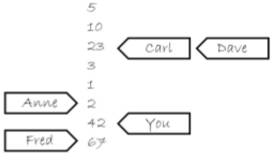
\includegraphics[width=0.7\textwidth]{relaxedOrdering.png}
                \end{center}
            \end{column}
        \end{columns}
        \begin{itemize}
            \item Переменная ``запомнит'', какое значение она вернула этому потоку
            \item Когда поток спросит значение в следующий раз, она вернёт ЛЮБОЕ значение между текущим и последним, которое она вернула ЭТОМУ потоку
        \end{itemize}
    \end{frame}

    \begin{frame}
        \frametitle{Interlocked}
        \begin{itemize}
            \item Одновременные чтение и запись в одной ``транзакции''
            \begin{itemize}
                \item \mintinline{fsharp}|Increment : location:int byref -> int|
                \item \mintinline{fsharp}|Decrement : location:int byref -> int|
                \item \mintinline{fsharp}|Add : location:int byref * value:int -> int|
                \item \mintinline{fsharp}|Exchange : location:int byref * value:int -> int|
                \item \mintinline{fsharp}|CompareExchange|
                        \mintinline{fsharp}|        : location:int byref * value:int * comparand:int -> int|
                \item \mintinline{fsharp}|Read : location:int64 byref -> int64| --- не нужен в x64
                \item \mintinline{fsharp}|MemoryBarrier : unit -> unit|
            \end{itemize}
        \end{itemize}
    \end{frame}

    \begin{frame}[fragile]
        \frametitle{Interlocked lock-free-максимум}
        \begin{footnotesize}
            \begin{minted}{fsharp}
let maximum (target: int ref) value =
    let mutable currentVal = !target
    let mutable startVal = 0
    let mutable desiredVal = 0
    let mutable isDone = false
    while not isDone do
        startVal <- currentVal
        desiredVal <- max startVal value
        // Тут другой поток мог уже испортить target, так что если она изменилась,
        // надо начать всё сначала.
        currentVal <- Interlocked.CompareExchange(target, desiredVal, startVal)
        if startVal = currentVal then
            isDone <- true
    desiredVal
            \end{minted}
        \end{footnotesize}
    \end{frame}

    \begin{frame}[fragile]
        \frametitle{Lock-free-список}
        \begin{footnotesize}
            \begin{minted}{fsharp}
type MutableList<'item when 'item: equality>(init) =
    let mutable items: 'item list = init

    member x.Value = items

    member x.Update updater =
        let current = items
        let newItems = updater current
        if not <| obj.ReferenceEquals
            (current, Interlocked.CompareExchange(&items, newItems, current))
            then x.Update updater
            else x

    member x.Add item = x.Update (fun l -> item :: l)
    member x.Remove item = x.Update (fun l -> List.filter (fun i -> i <> item) l)

    static member empty = new MutableList<'item>([])
            \end{minted}
            \attribution{\url{http://www.fssnip.net/ok}}
        \end{footnotesize}
    \end{frame}

    \begin{frame}
        \frametitle{Проблема ABA}
        \framesubtitle{Не всё так просто}
        \begin{enumerate}
            \item Поток 1 читает переменную x и видит A
            \item Поток 1 выполняет операцию над A
            \item Поток 1 засыпает
            \item Поток 2 выставляет значение x в B
            \item Поток 2 портит значение, ассоциированное с A
            \begin{itemize}
                \item Например, затирает запись с ключом A в хеш-таблице или удаляет файл A
            \end{itemize}
            \item Поток 2 меняет x назад в A, но ассоциирует с A новое значение 
            \begin{itemize}
                \item Например, добавляет новую запись или создаёт новый файл A
            \end{itemize}
            \item Поток 1 просыпается и выполняет CompareExchange, видя A
            \begin{itemize}
                \item Для него это то самое A, с которого он начал, так что всё падает
            \end{itemize}
        \end{enumerate}
    \end{frame}

    \begin{frame}[fragile]
        \frametitle{Пример}
        \begin{footnotesize}
            \begin{minted}{fsharp}
type LockFreeStack<'a>() =
    let mutable head: StackNode<'a> = Nil
    
    member this.Push (data: 'a) =
        let currentHead = head
        let newNode = Node(data, currentHead)
        if obj.ReferenceEquals
            (head, Interlocked.CompareExchange(&head, newNode, currentHead)) |> not 
            then this.Push (data)

    member this.Pop () =
        let currentHead = head
        match currentHead with
        | Nil -> failwith "Stack empty"
        | Node (data, next) ->
            if obj.ReferenceEquals
                (head, Interlocked.CompareExchange(&head, next, currentHead)) |> not 
            then this.Pop ()
            else data
            \end{minted}
        \end{footnotesize}
    \end{frame}

    \begin{frame}[fragile]
        \frametitle{Однако}
        \begin{minted}{fsharp}
let stack = LockFreeStack<int>()

Async.Start (async { 
    stack.Push 1
    stack.Push 2 // Тут засыпаем после let currentHead = head
})

// Тут просыпается поток 2
Async.Start (async { 
    stack.Pop () |> ignore // ...и скидывает 1
    stack.Push 3 // ...и кладёт на её место 3
})

// Поток 1 просыпается, ReferenceEquals true, и он затирает тройку
        \end{minted}
    \end{frame}

    \begin{frame}
        \frametitle{Итого}
        \begin{itemize}
            \item Lock-free --- когда несколько потоков могут получить доступ к структуре данных одновременно и гарантированно могут завершить операцию даже если остальные потоки сняты с исполнения
            \begin{itemize}
                \item Опасность \textit{голодания} --- один поток в цикле делает своё дело, второй в цикле пытется снова и снова, и не успевает
            \end{itemize}
            \item Wait-free --- это Lock-free плюс гарантия, что все потоки закончат работу за ограниченное число шагов
            \item Lock-free и wait-free-алгоритмы могут быть в разы эффективнее алгоритмов с блокировкой
            \item Но в сотни раз сложнее и труднее в сопровождении
            \item В общем: избегайте lock-free, если нет веских причин поступить иначе!
        \end{itemize}
    \end{frame}

\end{document}
